\documentclass[tikz,border=1pt]{standalone}
\usepackage[T1]{fontenc}
\usepackage{newtxtext}
\usepackage{newtxmath}
\usepackage{pgfplots}
\pgfplotsset{compat=1.18}

\definecolor{brevisLavender}{rgb}{0.924,0.921,0.987}
\definecolor{brevisMid}{HTML}{B9B2E5}
\definecolor{brevisMain}{HTML}{6758A8}
\definecolor{brevisDark}{HTML}{4B3F7E}
\definecolor{brevisInk}{HTML}{25324A}
\definecolor{brevisGrid}{HTML}{D9DDE4}

\begin{document}
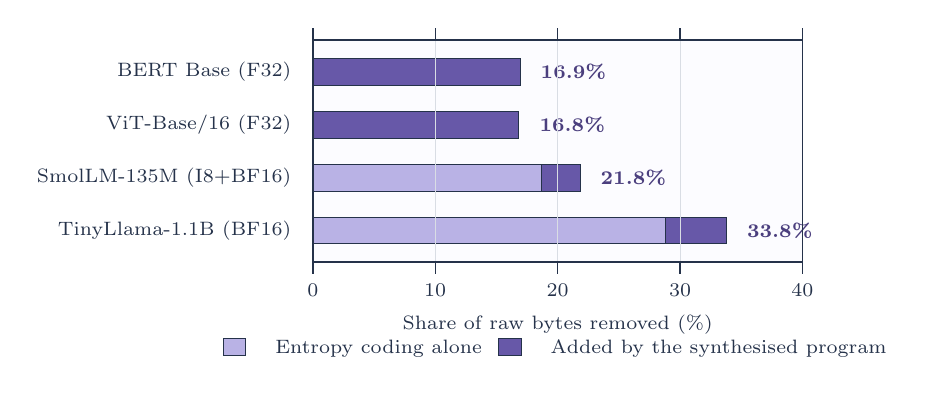
\begin{tikzpicture}
  \begin{axis}[
    width=78mm,
    height=44mm,
    xbar stacked,
    bar width=3.4mm,
    xmin=0,
    xmax=40,
    ymin=0.4,
    ymax=4.6,
    xtick={0,10,20,30,40},
    ytick={1,2,3,4},
    yticklabels={{BERT Base (F32)},{ViT-Base/16 (F32)},{SmolLM-135M (I8+BF16)},{TinyLlama-1.1B (BF16)}},
    y dir=reverse,
    xlabel={Share of raw bytes removed (\%)},
    axis lines=box,
    axis on top,
    tick align=outside,
    ytick style={draw=none},
    tick style={draw=brevisInk, line width=0.5pt},
    axis line style={draw=brevisInk, line width=0.6pt},
    xmajorgrids,
    ymajorgrids=false,
    major grid style={draw=brevisGrid, line width=0.32pt},
    axis background/.style={fill=brevisLavender!13},
    tick label style={font=\fontsize{6.8}{7.4}\selectfont,
      text=brevisInk},
    label style={font=\fontsize{7.1}{7.8}\selectfont,
      text=brevisInk},
    legend style={
      at={(0.5,-0.30)},
      anchor=north,
      legend columns=2,
      draw=none,
      fill=none,
      column sep=3mm,
      font=\fontsize{6.6}{7.2}\selectfont,
      text=brevisInk,
      /tikz/every even column/.append style={column sep=1.4mm},
    },
    clip=false,
  ]
    \addplot[fill=brevisMid, draw=brevisInk, line width=0.3pt]
      coordinates {(0.00,1) (0.00,2) (18.64,3) (28.81,4)};
    \addlegendentry{Entropy coding alone}
    \addplot[fill=brevisMain, draw=brevisInk, line width=0.3pt]
      coordinates {(16.92,1) (16.83,2) (3.18,3) (4.97,4)};
    \addlegendentry{Added by the synthesised program}

    \node[anchor=west, font=\bfseries\fontsize{6.6}{7.2}\selectfont, text=brevisDark] at (axis cs:17.82,1) {16.9\%};
    \node[anchor=west, font=\bfseries\fontsize{6.6}{7.2}\selectfont, text=brevisDark] at (axis cs:17.73,2) {16.8\%};
    \node[font=\fontsize{6.2}{6.8}\selectfont, text=brevisInk] at (axis cs:9.32,3) {18.6};
    \node[anchor=west, font=\bfseries\fontsize{6.6}{7.2}\selectfont, text=brevisDark] at (axis cs:22.72,3) {21.8\%};
    \node[font=\fontsize{6.2}{6.8}\selectfont, text=brevisInk] at (axis cs:14.40,4) {28.8};
    \node[anchor=west, font=\bfseries\fontsize{6.6}{7.2}\selectfont, text=brevisDark] at (axis cs:34.68,4) {33.8\%};
  \end{axis}
\end{tikzpicture}
\end{document}
